\chapter{Conditional Probability and Independence}

\section{Conditional probability}

Often we learn partial information about the outcome of an experiment and want to update
our probabilities. If we know $B$ has occurred, the only outcomes still possible are those
in $B$, so $B$ becomes the new sample space and we rescale.

\begin{definition}[Conditional probability]
For events $A$, $B$ with $P(B) > 0$, the \emph{conditional probability of $A$ given $B$}
is
\[
  P(A \given B) = \frac{P(A\cap B)}{P(B)}.
\]
\end{definition}

For fixed $B$, the function $A \mapsto P(A\given B)$ satisfies the three axioms, so all the
rules of Chapter 2 hold for conditional probabilities: for example
$P(\bar A\given B) = 1 - P(A\given B)$ and
$P(A_1\cup A_2 \given B) = P(A_1\given B) + P(A_2\given B) - P(A_1A_2\given B)$.

\begin{example}[Two dice]
Roll two fair dice. Let $A$ = ``sum is $8$'' and $B$ = ``first die shows $3$''.
$A\cap B = \{(3,5)\}$, so
\[
  P(A\given B) = \frac{1/36}{6/36} = \frac16, \qquad
  P(B\given A) = \frac{1/36}{5/36} = \frac15,
\]
since $A = \{(2,6),(3,5),(4,4),(5,3),(6,2)\}$. Note $P(A\given B) \ne P(B\given A)$ in
general.
\end{example}

\begin{example}[Children]
A family has two children, each equally likely to be a boy or girl independently. Given
that at least one is a girl, what is the probability both are girls? With
$S = \{BB,BG,GB,GG\}$,
\[
  P(GG \given \text{at least one } G) = \frac{1/4}{3/4} = \frac13,
\]
not $1/2$, which is a classic trap.
\end{example}

\section{The product rule}

Rearranging the definition gives a way to compute probabilities of intersections in
stages.

\begin{theorem}[Product (multiplication) rule]
For events with positive probabilities,
\[
  P(AB) = P(A)\,P(B\given A),
\]
and more generally
\[
  P(A_1A_2\cdots A_n) = P(A_1)\,P(A_2\given A_1)\,P(A_3\given A_1A_2)\cdots
  P(A_n\given A_1\cdots A_{n-1}).
\]
\end{theorem}

\begin{proof}
The two-event case is the definition multiplied out. For $n$ events, the right side
telescopes: each factor $P(A_k\given A_1\cdots A_{k-1}) = P(A_1\cdots A_k)/P(A_1\cdots A_{k-1})$.
\end{proof}

\begin{example}[Three hearts]
Three cards are dealt without replacement. Let $H_i$ = ``card $i$ is a heart''. Then
\[
  P(H_1H_2H_3) = \frac{13}{52}\cdot\frac{12}{51}\cdot\frac{11}{50} = \frac{1716}{132\,600}
  \approx 0.01294,
\]
which agrees with the counting answer $\binom{13}3/\binom{52}3 = 286/22\,100$.
\end{example}

\section{The law of total probability and Bayes' theorem}

\begin{definition}[Partition]
Events $B_1, \dots, B_k$ form a \emph{partition} of $S$ if they are pairwise mutually
exclusive and $B_1\cup\cdots\cup B_k = S$.
\end{definition}

\begin{theorem}[Law of total probability]
If $B_1,\dots,B_k$ partition $S$ and each $P(B_i)>0$, then for any event $A$,
\[
  P(A) = \sum_{i=1}^k P(A\given B_i)\,P(B_i).
\]
\end{theorem}

\begin{proof}
$A = AB_1 \cup \cdots \cup AB_k$ is a disjoint union, so $P(A) = \sum_i P(AB_i)$, and
$P(AB_i) = P(A\given B_i)P(B_i)$ by the product rule.
\end{proof}

The simplest partition is $\{B, \bar B\}$:
$P(A) = P(A\given B)P(B) + P(A\given \bar B)P(\bar B)$.

\begin{theorem}[Bayes' theorem]
If $B_1,\dots,B_k$ partition $S$, then for any $A$ with $P(A)>0$,
\[
  P(B_j\given A) = \frac{P(A\given B_j)P(B_j)}{\sum_{i=1}^k P(A\given B_i)P(B_i)}.
\]
In particular $P(B\given A) = \dfrac{P(A\given B)P(B)}{P(A\given B)P(B) + P(A\given\bar B)P(\bar B)}$.
\end{theorem}

\begin{proof}
$P(B_j\given A) = P(AB_j)/P(A)$; write the numerator with the product rule and the
denominator with the law of total probability.
\end{proof}

Bayes' theorem ``reverses'' the conditioning: we usually know $P(\text{evidence}\given
\text{cause})$ and want $P(\text{cause}\given\text{evidence})$. A tree diagram is the
easiest way to organise these calculations.

\begin{example}[Medical test]
A disease affects $1\%$ of a population. A test detects the disease in $95\%$ of people
who have it (sensitivity) and gives a false positive for $5\%$ of people who do not. A
randomly chosen person tests positive. What is the probability they have the disease?

Let $D$ = ``has disease'' and $+$ = ``tests positive''.
\[
  P(+) = P(+\given D)P(D) + P(+\given\bar D)P(\bar D) = (0.95)(0.01) + (0.05)(0.99)
  = 0.0095 + 0.0495 = 0.059,
\]
\[
  P(D\given +) = \frac{0.0095}{0.059} \approx 0.161.
\]
Only about $16\%$ of positives actually have the disease! Because the disease is rare, the
false positives from the large healthy group swamp the true positives. Ignoring the
prior $P(D)$ is called the \emph{base rate fallacy}.
\end{example}

\begin{center}
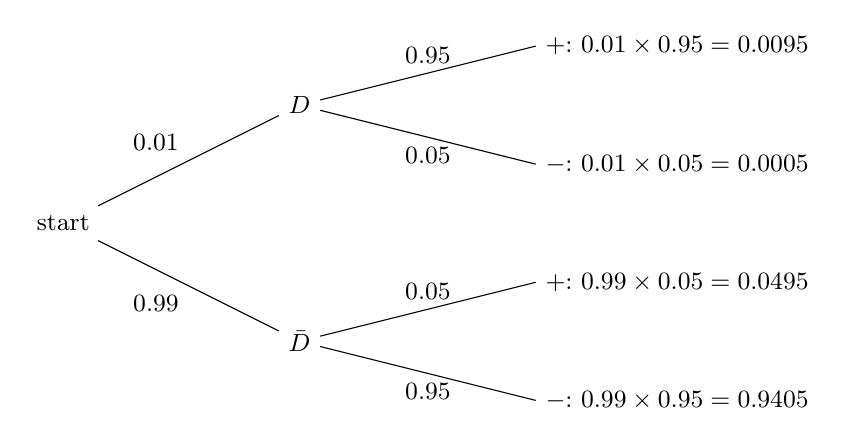
\begin{tikzpicture}[every node/.style={font=\small}]
  \node (s) at (0,0) {start};
  \node (D) at (3,1.5) {$D$};
  \node (N) at (3,-1.5) {$\bar D$};
  \node[anchor=west] (Dp) at (6,2.25) {$+$:\ $0.01\times0.95 = 0.0095$};
  \node[anchor=west] (Dm) at (6,0.75) {$-$:\ $0.01\times0.05 = 0.0005$};
  \node[anchor=west] (Np) at (6,-0.75) {$+$:\ $0.99\times0.05 = 0.0495$};
  \node[anchor=west] (Nm) at (6,-2.25) {$-$:\ $0.99\times0.95 = 0.9405$};
  \draw (s) -- node[above left] {$0.01$} (D);
  \draw (s) -- node[below left] {$0.99$} (N);
  \draw (D) -- node[above] {$0.95$} (Dp.west);
  \draw (D) -- node[below] {$0.05$} (Dm.west);
  \draw (N) -- node[above] {$0.05$} (Np.west);
  \draw (N) -- node[below] {$0.95$} (Nm.west);
\end{tikzpicture}
\end{center}

\begin{example}[Three machines]
Machines $M_1, M_2, M_3$ produce $50\%$, $30\%$, $20\%$ of a factory's output, with defect
rates $1\%$, $2\%$, $3\%$ respectively. Then
\[
  P(\text{defective}) = (0.5)(0.01) + (0.3)(0.02) + (0.2)(0.03) = 0.005 + 0.006 + 0.006
  = 0.017.
\]
Given that an item is defective, the probability it came from $M_3$ is
$0.006/0.017 = 6/17 \approx 0.353$, and from $M_1$ it is $5/17 \approx 0.294$. So
although $M_1$ makes the most items, a defective item is most likely to come from $M_3$
(tied with $M_2$ at $6/17$).
\end{example}

\begin{example}[Monty Hall]
A prize is behind one of three doors. You pick door $1$; the host, who knows where the
prize is, opens one of the other doors that hides no prize (choosing at random if both
are empty), say door $3$. Should you switch to door $2$? Let $C_i$ = ``prize behind door
$i$'' and $O_3$ = ``host opens door $3$''. Then $P(O_3\given C_1) = 1/2$,
$P(O_3\given C_2) = 1$, $P(O_3\given C_3) = 0$, so
\[
  P(C_2\given O_3) = \frac{1\cdot\frac13}{\frac12\cdot\frac13 + 1\cdot\frac13 + 0} =
  \frac{2}{3}.
\]
Switching wins with probability $2/3$.
\end{example}

\section{Independence}

\begin{definition}[Independent events]
Events $A$ and $B$ are \emph{independent} if
\[
  P(AB) = P(A)\,P(B).
\]
\end{definition}

When $P(B)>0$ this is equivalent to $P(A\given B) = P(A)$: knowing $B$ occurred does not
change the probability of $A$. The product form is preferred as the definition because it
is symmetric and also makes sense when $P(B)=0$.

\begin{theorem}
If $A$ and $B$ are independent, then so are $A$ and $\bar B$, $\bar A$ and $B$, and
$\bar A$ and $\bar B$.
\end{theorem}

\begin{proof}
$P(A\bar B) = P(A) - P(AB) = P(A) - P(A)P(B) = P(A)(1 - P(B)) = P(A)P(\bar B)$. The other
cases follow by symmetry and by applying this twice.
\end{proof}

\begin{example}
Roll one fair die; let $A = \{2,4,6\}$ (even) and $B = \{1,2\}$. Then
$P(AB) = P(\{2\}) = 1/6 = (1/2)(1/3) = P(A)P(B)$, so $A$, $B$ are independent, even
though they come from a single roll. With $B' = \{1,2,3\}$ instead,
$P(AB') = 1/6 \ne (1/2)(1/2)$, so $A$ and $B'$ are dependent.
\end{example}

\begin{important}[Independent vs.\ mutually exclusive]
If $A$ and $B$ are mutually exclusive with $P(A), P(B) > 0$, then $P(AB) = 0 \ne
P(A)P(B)$, so they are \emph{dependent}: knowing $A$ occurred tells you $B$ did not.
\end{important}

\subsection{Independence of several events}

\begin{definition}[Mutual independence]
Events $A_1,\dots,A_n$ are \emph{(mutually) independent} if for every subcollection
$A_{i_1},\dots,A_{i_k}$ with $2 \le k \le n$,
\[
  P(A_{i_1}A_{i_2}\cdots A_{i_k}) = P(A_{i_1})P(A_{i_2})\cdots P(A_{i_k}).
\]
They are \emph{pairwise independent} if this holds for all pairs ($k=2$).
\end{definition}

For three events, mutual independence requires all four equations
$P(AB) = P(A)P(B)$, $P(AC) = P(A)P(C)$, $P(BC) = P(B)P(C)$ and
$P(ABC) = P(A)P(B)P(C)$.

\begin{example}[Pairwise but not mutually independent]
Toss two fair coins. Let $A$ = ``first is H'', $B$ = ``second is H'', $C$ = ``both coins
show the same face''. Then $P(A)=P(B)=P(C) = 1/2$ and
\[
  P(AB) = P(\{HH\}) = \tfrac14,\quad P(AC) = P(\{HH\}) = \tfrac14,\quad
  P(BC) = P(\{HH\}) = \tfrac14,
\]
so the events are pairwise independent. But $P(ABC) = P(\{HH\}) = 1/4 \ne 1/8$: any two
of them determine the third, so they are not mutually independent.
\end{example}

\begin{example}[System reliability]
Each component of a system works independently with probability $0.9$.
\begin{itemize}
  \item Three components \emph{in series} (all must work):
        $P(\text{works}) = 0.9^3 = 0.729$.
  \item Three components \emph{in parallel} (at least one must work):
        $P(\text{works}) = 1 - P(\text{all fail}) = 1 - 0.1^3 = 0.999$.
  \item Two parallel pairs connected in series:
        $(1 - 0.1^2)^2 = 0.99^2 = 0.9801$.
\end{itemize}
\end{example}

\section{Common pitfalls}

\begin{itemize}
  \item $P(A\given B)$ and $P(B\given A)$ are different (``prosecutor's fallacy'').
  \item Independence must be justified (physically separate experiments) or verified with
        the product formula; it cannot be read off a Venn diagram.
  \item Draws \emph{without} replacement are dependent; draws \emph{with} replacement are
        independent.
\end{itemize}

\section{Summary}

\begin{itemize}
  \item $P(A\given B) = P(AB)/P(B)$; conditional probabilities obey all the usual rules.
  \item Product rule: $P(AB) = P(A)P(B\given A)$, extended to chains of events.
  \item Total probability: $P(A) = \sum_i P(A\given B_i)P(B_i)$ over a partition.
  \item Bayes: $P(B_j\given A) = P(A\given B_j)P(B_j)/P(A)$.
  \item Independence: $P(AB) = P(A)P(B)$; complements of independent events are
        independent; mutual independence needs all sub-products, and is strictly
        stronger than pairwise independence.
\end{itemize}
